% !TEX program = XeLaTeX
\documentclass[12pt, a4paper, oneside]{book}
\usepackage{amsmath}
\usepackage{amssymb}
\usepackage{graphicx}
\usepackage{fontspec}
\usepackage{float}
\usepackage{ltablex} % Thay tabularx bằng ltablex để hỗ trợ ngắt trang
\usepackage[hyphens]{url} 
\usepackage[colorlinks=true, linkcolor=blue, urlcolor=blue]{hyperref}

\graphicspath{{assets/}}

% Cấu hình ltablex để căn giữa nội dung
\newcolumntype{C}{>{\centering\arraybackslash}X}
\keepXColumns % Giữ tính năng tự dãn của tabularx cho longtable

% --- KHAI BÁO NEWCOMMAND ---
\newcommand{\paperrow}[4]{%
    #1 & 
    \href{#2}{Paper Link} & 
    \href{#3}{Source Code} & 
    \hyperlink{#4}{Architecture} \tabularnewline \hline
}

\begin{document}

\chapter{Paper}

% Không dùng môi trường \begin{table} nữa, dùng trực tiếp tabularx (đã được ltablex nâng cấp)
\renewcommand{\arraystretch}{2.2}
\begin{tabularx}{\textwidth}{|C|C|C|C|}
    \hline
    \textbf{Model Name} & \textbf{Link Paper} & \textbf{Source Code} & \textbf{Architecture} \tabularnewline
    \hline

    \paperrow{BiomedCoOp \textbf{(main paper)}}{https://arxiv.org/abs/2411.15232}{https://github.com/HealthX-Lab/BiomedCoOp}{fig:biomed_arch}

    \paperrow{VPT \textbf{(Vision Prompt Tuning)}}{https://arxiv.org/abs/2203.12119}{https://github.com/kmnp/vpt}{fig:VPT_arch}
    
    \paperrow{MeDKCoOp \textbf{(Dual Knowledge)}}{https://dl.acm.org/doi/10.1145/3746027.3755135}{https://github.com/WangYijun-OUC/MeDKCoOp}{fig:MeDK_arch}
    
    \paperrow{DPT \textbf{(Dual Modality Prompt Tuning)}}{https://arxiv.org/abs/2208.08340}{https://github.com/fanrena/DPT}{fig:dpt_arch} 
    
    \paperrow{Biomed-DPT \textbf{(Dual Modality)}}{https://arxiv.org/abs/2505.05189}{https://github.com/Kanyooo/Biomed-DPT}{fig:B_DPT_arch}
    
    \paperrow{Prompt SRC \textbf{(Self-regulating)}}{https://arxiv.org/abs/2307.06948}{https://github.com/muzairkhattak/PromptSRC}{fig:SRC_arch}
    
    \paperrow{MaPLe \textbf{(Multi-modal)}}{https://arxiv.org/abs/2210.03117}{https://github.com/muzairkhattak/multimodal-prompt-learning}{fig:MaPLe_arch}

    \paperrow{MedGemma}{https://arxiv.org/abs/2507.05201}{}{}

    \paperrow{XCoOp}{https://arxiv.org/abs/2403.09410}{}{}
\end{tabularx}


\chapter{Model Architecture}

\begin{figure}[H]
    \centering
    \hypertarget{fig:biomed_arch}{}
    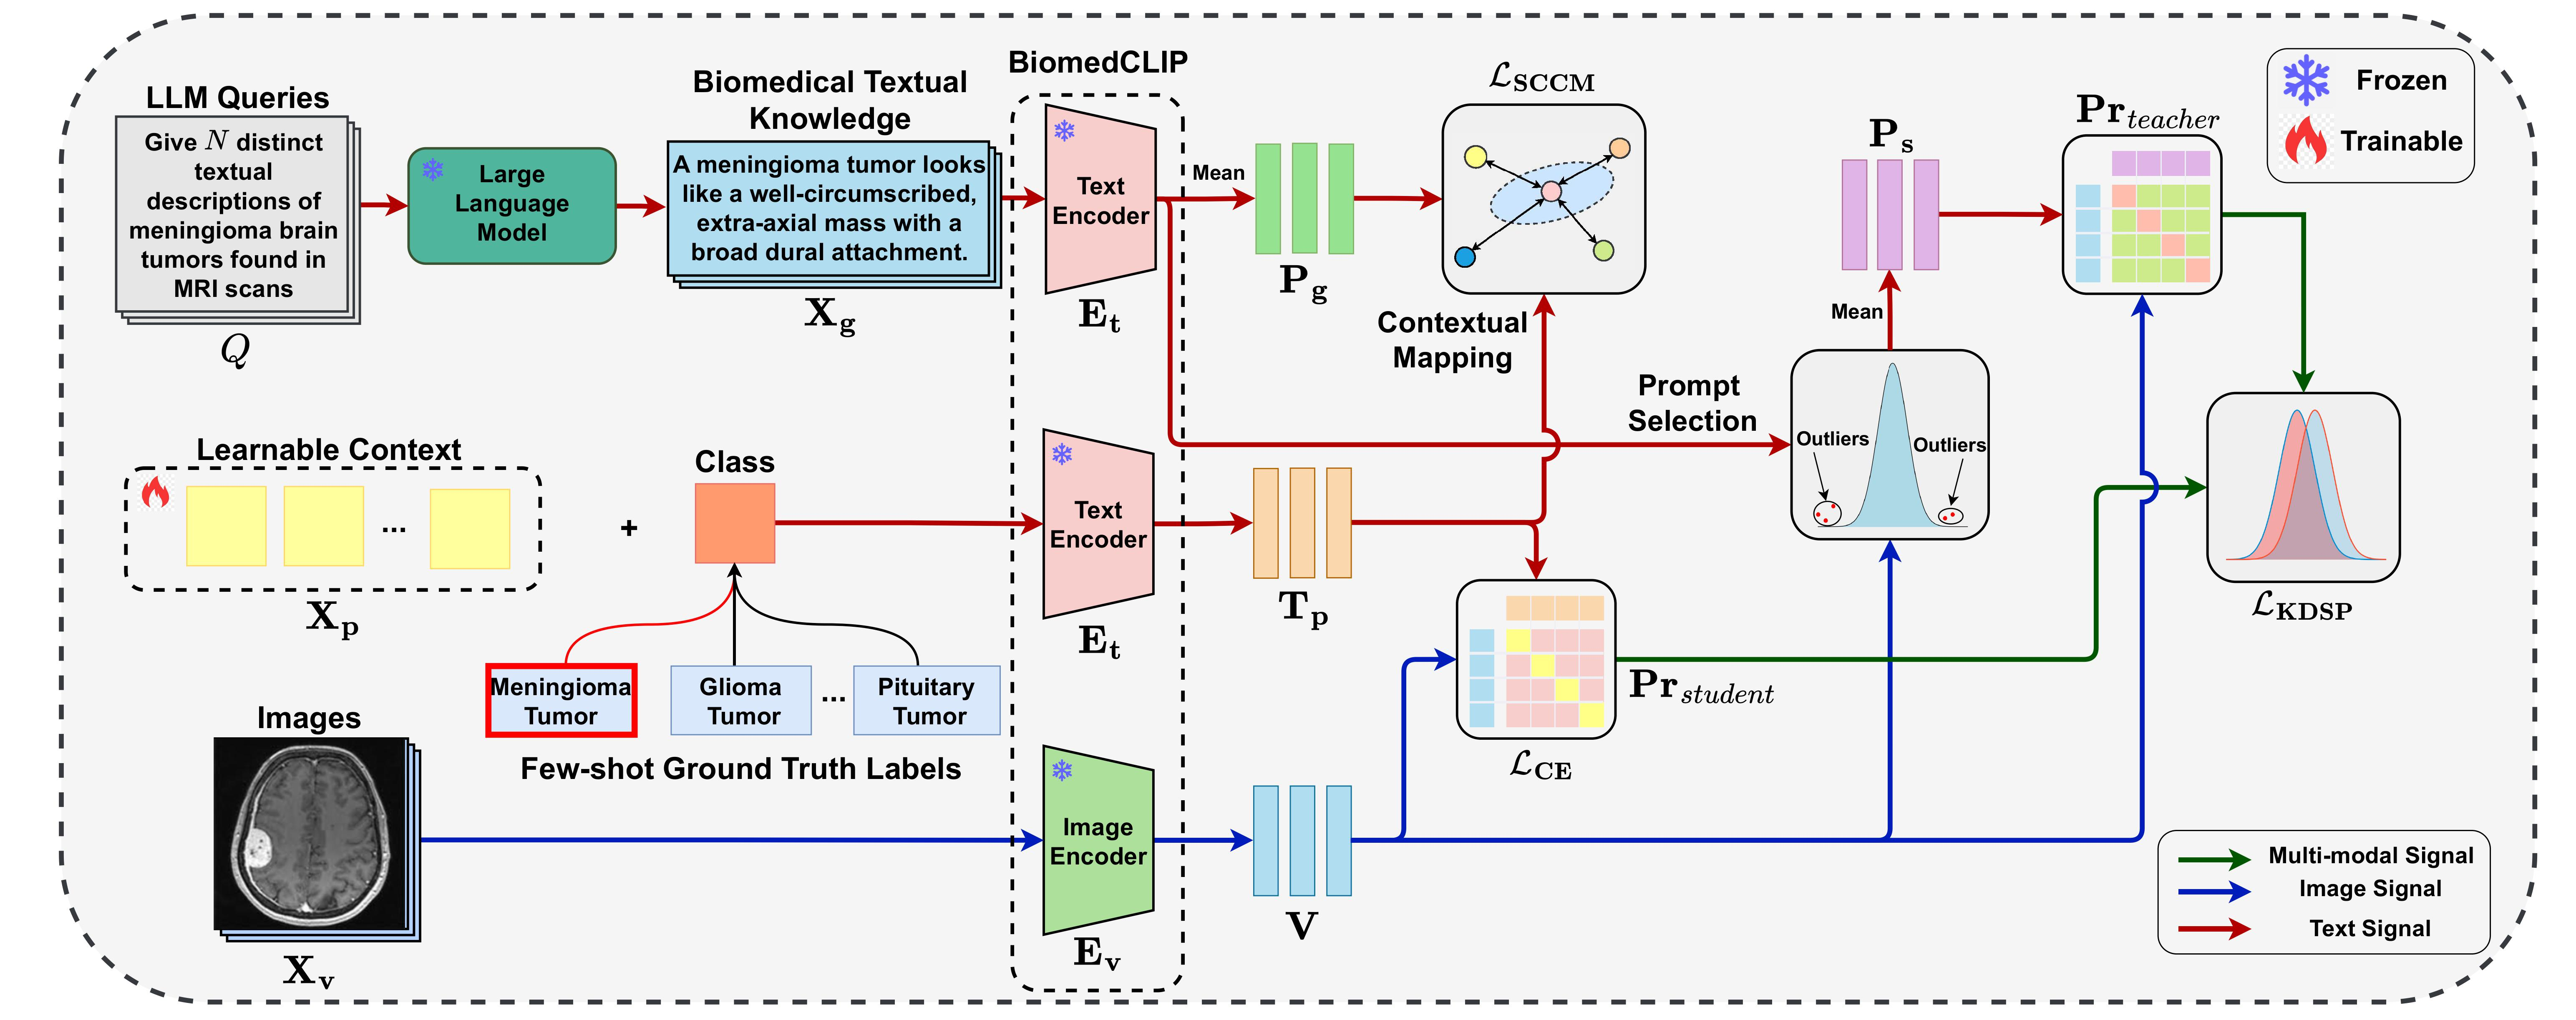
\includegraphics[width=1.25\textwidth]{BiomedCoOp.jpg} 
    \caption{BiomedCoOp Architecture}
\end{figure}

\begin{figure}[H]
    \centering
    \hypertarget{fig:VPT_arch}{}
    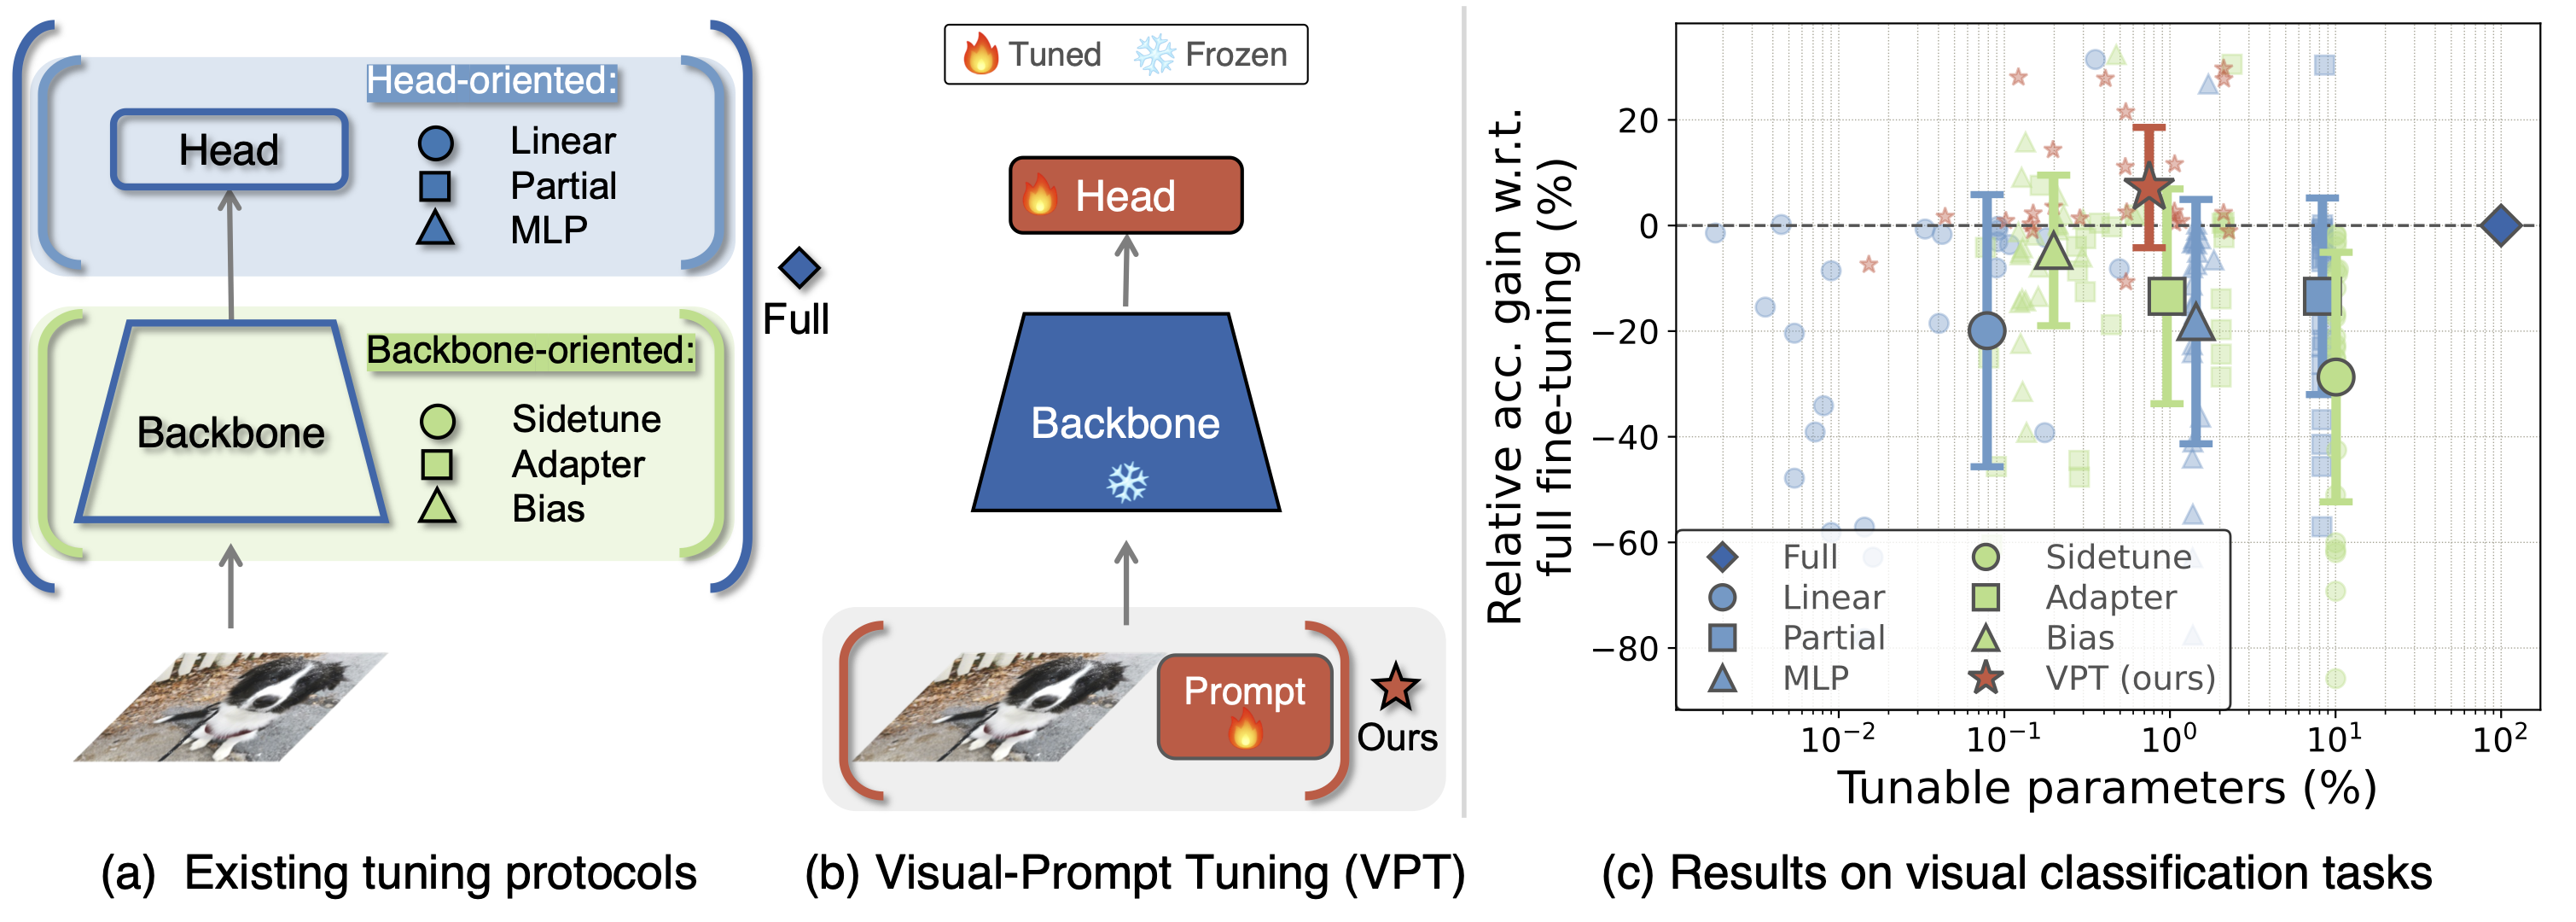
\includegraphics[width=1.25\textwidth]{VisionPromptTuning.png}
    \caption{Vision Prompt Tuning Architecture}
\end{figure}

\begin{figure}[H]
    \centering
    \hypertarget{fig:MeDK_arch}{}
    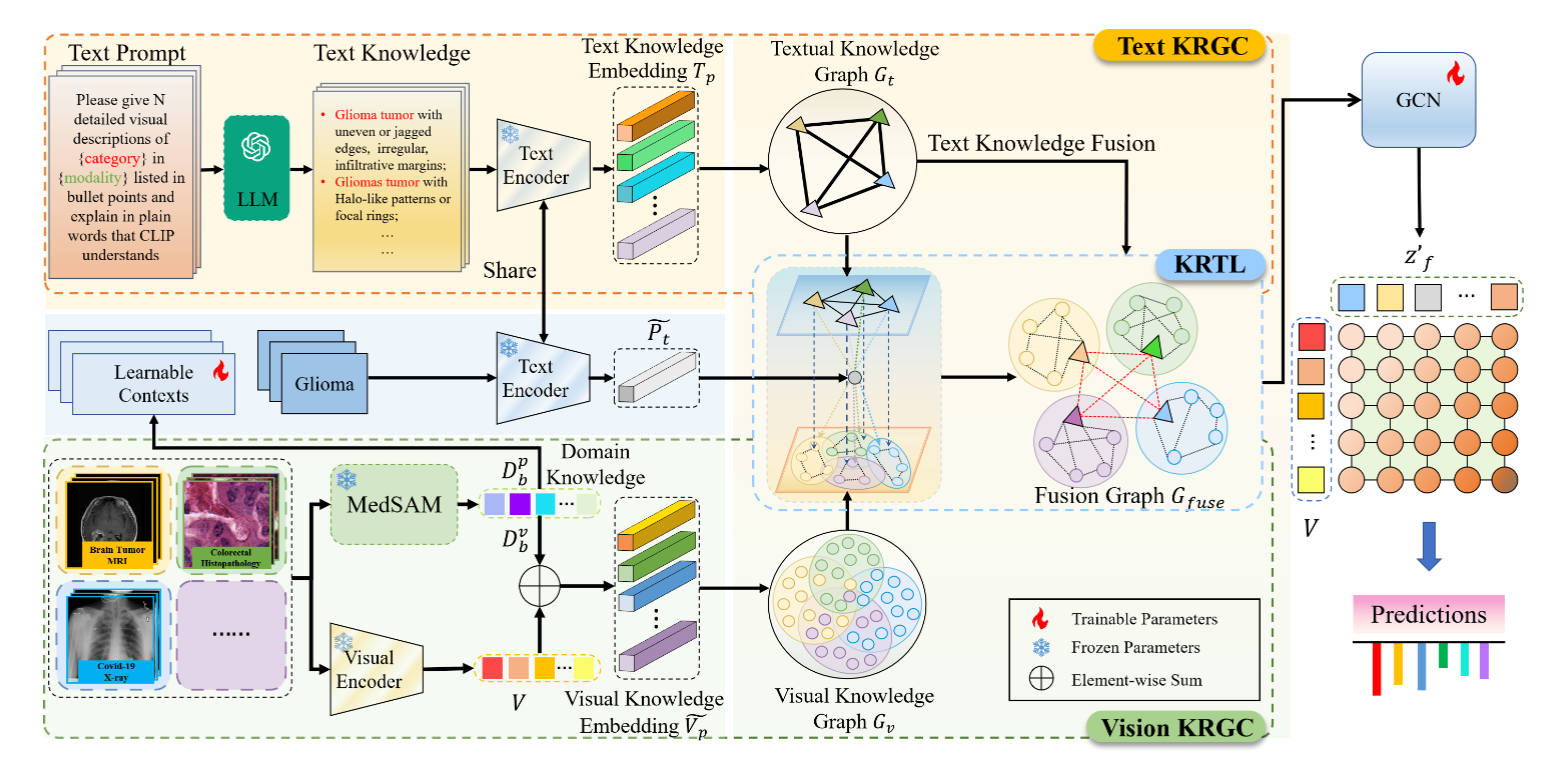
\includegraphics[width=1.25\textwidth]{MeDKCoOp.png}
    \caption{MeDKCoOp Architecture}
\end{figure}

\begin{figure}[H]
    \centering
    \hypertarget{fig:dpt_arch}{}
    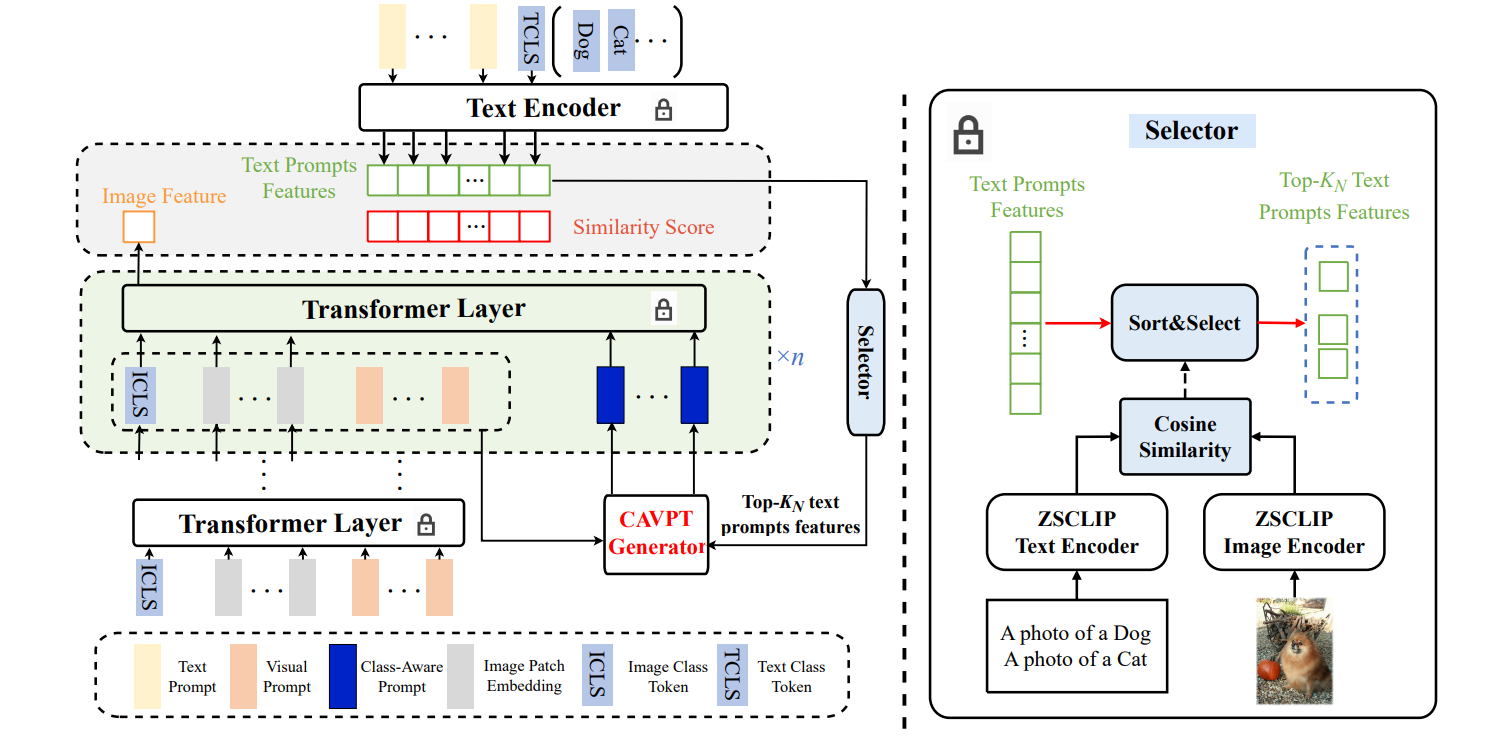
\includegraphics[width=1.25\textwidth]{DualModabilityPrompt.png}
    \caption{Dual Modality Prompt Tuning Architecture}
\end{figure}


\begin{figure}[H]
    \centering
    \hypertarget{fig:B_DPT_arch}{}
    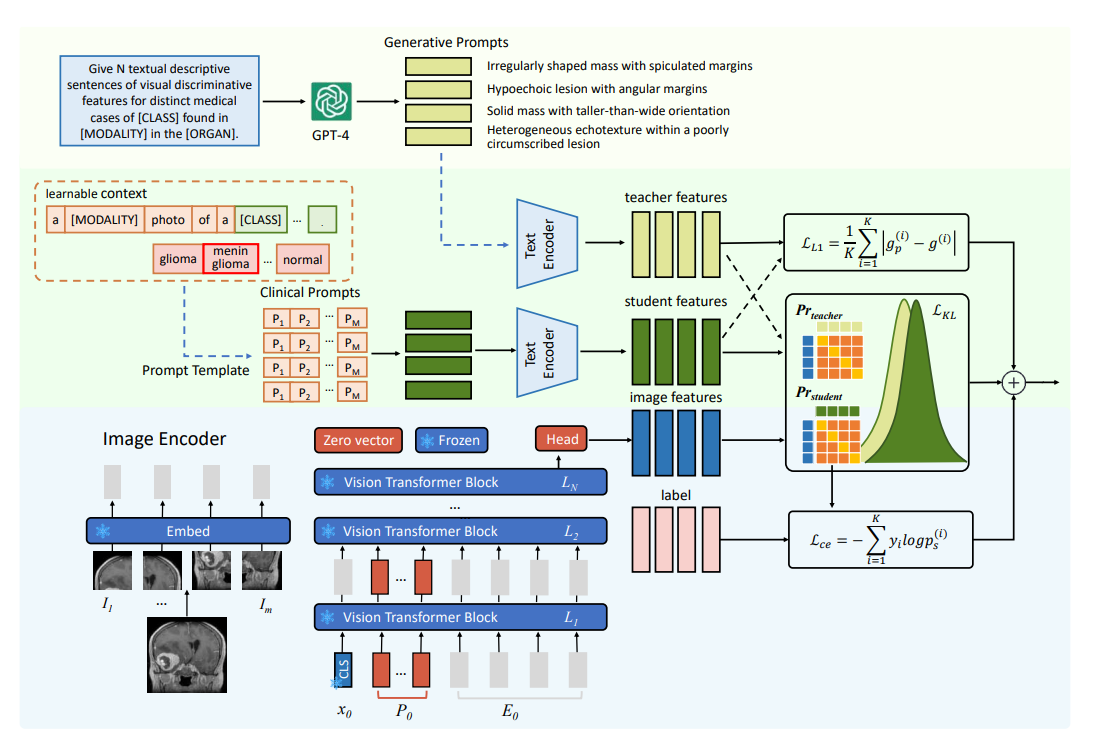
\includegraphics[width=1.25\textwidth]{Biomedical-VPT.png}
    \caption{Biomed-DPT Architecture}
\end{figure}

\begin{figure}[H]
    \centering
    \hypertarget{fig:SRC_arch}{}
    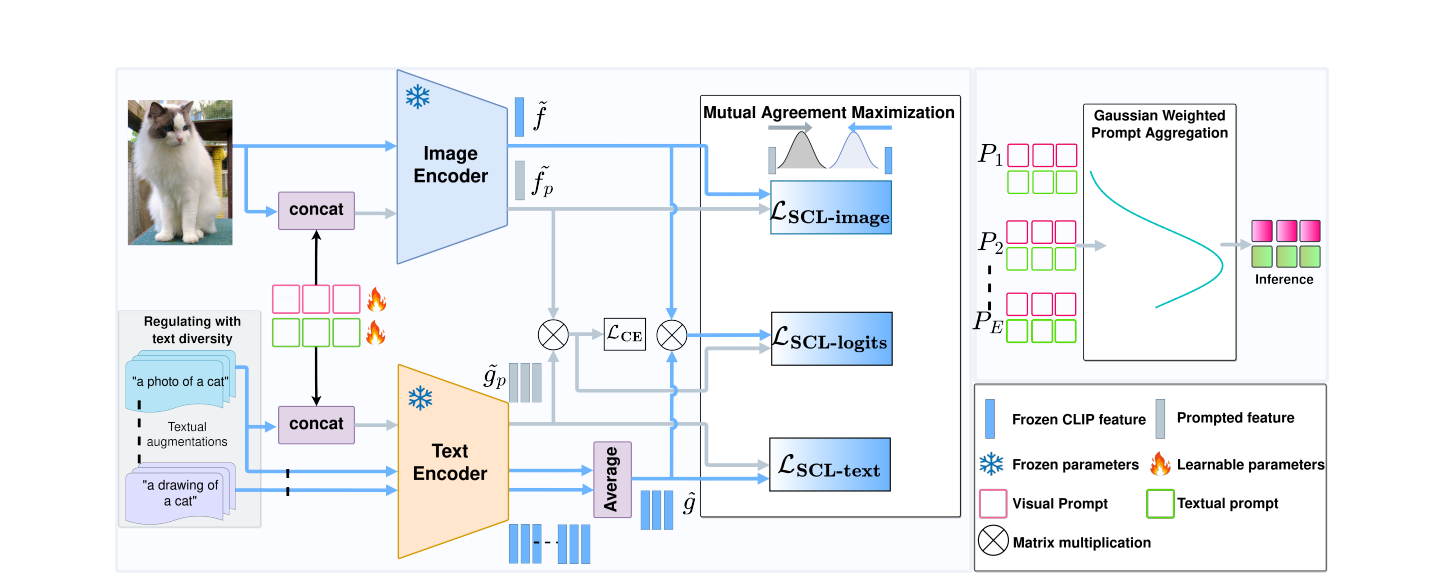
\includegraphics[width=1.25\textwidth]{SRC.png}
    \caption{SRC Architecture}
\end{figure}

\begin{figure}[H]
    \centering
    \hypertarget{fig:MaPLe_arch}{}
    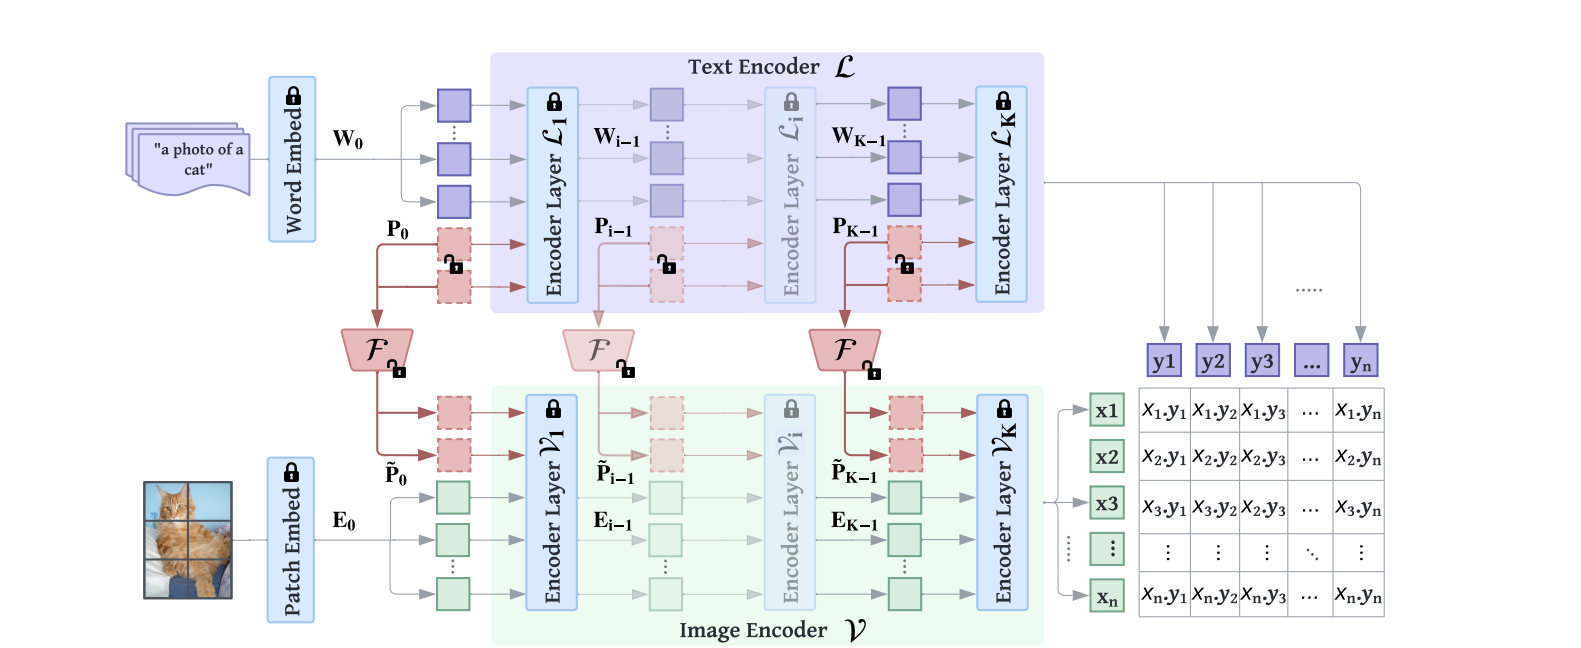
\includegraphics[width=1.25\textwidth]{MaPLe.png}
    \caption{MaPLe Architecture}
\end{figure}


\end{document}